\subsection{Incorporating Helium into the DEM Framework}\label{sec:cfdem-heat-transfer}

In the standard DEM implementation (see \cref{sec:particle-dynamics}), each pebble obeys Newton's equations of motion in response to a net force acting upon it. To include the influence of helium in the DEM formulation, we simply add a drag force term to Eq.~\ref{eq:newton-translational}. The momentum balance of our Lagrangian-tracked pebble now reads,
\begin{equation}\label{eq:cfdem-dem-momentum}
	m_i  \ddt{\vec{r}_i} = m_i\vec{g} + \vec{f}_i + \beta_i V_i \Delta \vec{u}_{if}
\end{equation}
where all but the last term is identical to Eq.~\ref{eq:newton-translational}. The components of the last term are $\Delta \vec{u}_{if} = \vec{u}_f - u_i$, which is the relative velocity between the fluid and pebble, $i$; $\beta_i$, which is the inter-phase momentum exchange coefficient; and the drag acts upon the entire pebble volume, $V_i$. A discussion on the method of determination and form of the inter-phase drag coefficient will be discussed after introducing the DEM heat transfer equation.

To similarly include the influence of the interstitial helium on the temperatures of our pebbles, we must simply add a source term to the original energy balance equation of the DEM pebble, as given in Eq.~\ref{eq:thermoFirstLaw}. The inter-phase energy exchange coefficient (using consistent syntax with the momentum equation) is actually just the standard heat transfer coefficient, $h$, for a fluid moving past a sphere in a packed bed. After adding the inter-phase energy exchange coefficient, the energy balance of the particle now reads,
\begin{equation}\label{eq:cfdem-dem-energy}
	m_iC_i \ddt{T_i} = Q_{s,i} + \sum_{j=1}^Z Q_{ij} + h_i A_i \Delta T_{if}
\end{equation}
where again we have only needed to add the last term to account for the energy deposited/removed by the passing fluid. $\Delta T_{if}$ is the temperature difference, $T_f - T_i$, and the inter-phase energy exchange coefficient, $h_i$, acts upon the pebble surface area, $A_i$.

In the development of Eq.~\ref{eq:thermoFirstLaw}, it was assumed that a `conduction' Biot number was satisfied such that a lumped-capacitance method would be valid for the discrete pebbles in our ensemble. Likewise, for Eq.~\ref{eq:cfdem-dem-energy} to be valid, we must assume that the true Biot number is also $\Bi \ll 1$. However, the lumped capacitance method is generally developed in heat transfer systems without heat generation. Furthermore, considering the low conductivity of our pebble material, it is not apparent \textit{a priori} if the lumped capacitance assumption inherent in our DEM formulation is valid. I return to explore this issue in \cref{sec:ht-jeffreson-correction}.

Assuming their validity, these simple additions to the governing equations of momentum and energy of each particle are all that are necessary to incorporate helium into the DEM computations. The computations of the inter-phase exchange coefficients, $\beta_i$ and $h_i$ are discussed next.

\subsection{Inter-phase Exchange Coefficients}

The purge gas in ceramic breeders is meant to travel at very low flow rates to maximize the absorption of tritium. Furthermore, the pebble beds will always be near the close-packed limit. As such, the particle Reynolds number for these flows is often near unity and the Kozeny-Carman equation as applicable for Stokes flow is quite sufficient. However, we will employ the full Koch-Hill-Ladd (KHL) correlations which include terms for both the Stokes flow correlation (as a function of $\phi$) in the zero Reynolds number limit and the viscous effects with a Reynolds number-dependent term. The KHL correlation is of a general form, and reduces to the Kozeny-Carman correlation in the close-packed, zero Reynolds number limits.\cite{Koch2001} The nondimensional force of the KHL correlation reads,
\begin{equation}\label{eq:khl-correlation}
	F = F_0(\phi) + F_3(\phi)\Re
\end{equation}
where the viscous term of the drag is
\begin{equation}
F_0 = \begin{cases}
	\frac{1+3(\phi/2)^{1/2} + (135/64)\phi\ln\phi + 16.14\phi}{1 + 0.681\phi - 8.48 \phi^2 + 8.16\phi^3} & \text{if $\phi < 0.4$}\\
	10.0\,\frac{\phi}{(1-\phi)^3} & \text{if $\phi > 0.4$} 
	\end{cases}
\end{equation}
and the inertial component of the drag is
\begin{equation}
	F_3 = 0.0673 + 0.212\phi + 0.0232 \frac{1}{(1-\phi)^5}
\end{equation}

The correlation from Koch-Hill-Ladd provide a nondimensional drag that must simply be re-written to fit into the pattern of our inter-phase momentum exchange coefficient. The momentum exchange coefficient follows the common form by Gidaspow\cite{gidaspow1994multiphase} (actually differing from that used here by a factor of $1-\phi$ due to definitions of pressure and buoyancy in the drag force) thus,\cite{Hoef2005,Benyahia2006}
\begin{equation}\label{eq:interphase-momentum}
	\beta_{i} = \frac{18\mu_f}{d_{p,i}^2}(1-\phi_k)\phi_k F
\end{equation}
where $\mu_f$ is the fluid viscosity and the diameter of pebble $i$ is $d_{p,i}$. The packing fraction, $\phi_k$, in this equation is the local packing fraction in the fluid cell $k$. This value will differ from the global/bulk value in near-wall regions. As a short aside, container walls have long been known to theoretically and experimentally force order to the packing regardless of shape of packing.\cite{Hunt1990,Benenati1962,Baird1958} For example, the void fraction ($\epsilon = 1-\phi$) in narrow annular containers using the correlation from Mueller, as a function of wall-distance in a cylinder is,\cite{Mueller1999}
\[
\epsilon = \epsilon_0 + (1-\epsilon_0)J_0(ar^*)e^{-br^*}
\]
where $r^*$ is the nondimensional distance from the wall; here it is defined in terms of the pebble diameter, $r^* = r/d_p$. The constants, a and b, are defined in terms of the size parameter $\alpha = D/d_p$ where $D$ is the diameter of the annular tube. First, $a$ is
\[
    a= 
\begin{cases}
    7.383 - \cfrac{2.932}{\alpha - 9.864}, & \text{if }\  \alpha \geq 13\\
    8.243 - \cfrac{12.98}{\alpha + 3.156}, & \text{if} \ 13 \geq \alpha \geq 2.61
\end{cases}
\]
then
\[
b = 0.304 - \cfrac{0.724}{\alpha}
\]
The bulk void fraction is found from the correlation:
\[
\epsilon_0 = 0.379 + \cfrac{0.078}{\alpha - 1.8}
\]

The packing fractions as a function of distance from the container wall for two example sizes, diameters of 20$d_p$ and 5$d_p$, are plotted in Fig.~\ref{fig:packingDist}. This example is meant to demonstrate the varying packing fraction in a packed bed that is described with a single `bulk' or `global' packing fraction. The size of the discretized cell relative to the pebble will dictate how much of the void fraction variation is captured in the volume-averaged equations.

\begin{figure}[htbp]
\begin{center}
	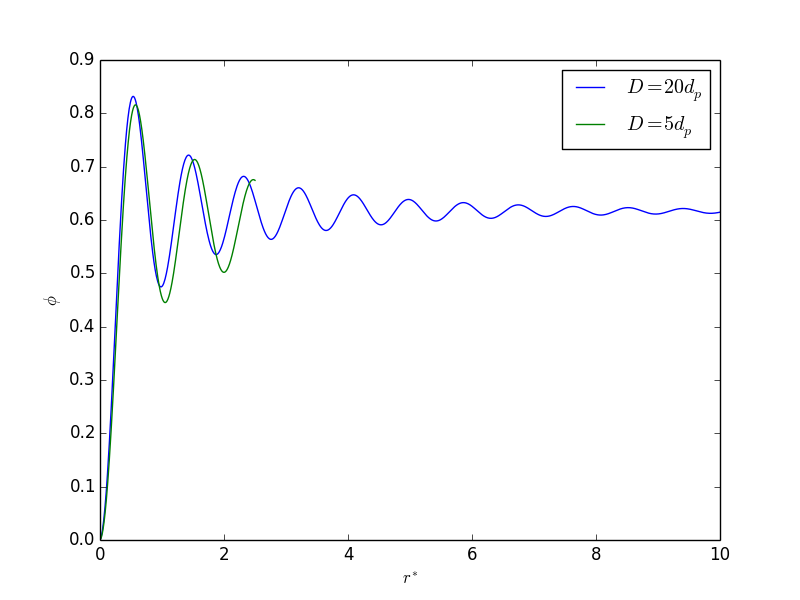
\includegraphics[width = \singleimagewidth]{chapters/figures/annular-packing-fraction.png}
	\caption{Showing the packing fraction approach the bulk value after a few pebble diameters when the pipe is 20$d_p$ and that when the pipe is only 5$d_p$, the packing fraction at any radius is not the same as the bed average.}
	\label{fig:packingDist}
\end{center}
\end{figure}

The correlation we have used here is just one possible option of many that have been developed historically for estimating the pressure drop / permeability / drag force of fluid in a packed bed. A short review of other correlations, their applicable ranges of fluid parameters, and other details is given in \cref{sec:modeling-pressure-drop}. The assumptions leading to Eq.~\ref{eq:K-C-non-dim} provide justification for our implementation of the KHL correlation for our packed beds of lithium ceramics.
\FloatBarrier



The inter-phase energy transfer coefficient is calculated from the Nusselt number for the helium flow in the ensemble,
\begin{equation}\label{eq:interphase-energy}
	h_i = \frac{\Nu k_f}{d_{p,i}}
\end{equation}
where $k_f$ is the thermal conductivity of the fluid. Several correlations for determining the Nusselt number are given for reference in \cref{sec:particle-convection}. We opt for the correlation provided by Li \& Mason which is applicable to a wide range of Reynolds number flows.\cite{Li2000} Their correlation reads,
\begin{equation}\label{eq:li-mason-correlation}
	\Nu = \begin{cases}
	2+ 0.6\epsilon^n\Re_p^{1/2}\Pr^{1/3} 										& \Re_p < 200\\
	2+ 0.5\epsilon^n\Re_p^{1/2}\Pr^{1/3} + 0.02 \epsilon^n \Re_p^{0.8}\Pr^{1/3} & 200 < \Re_p < 1500\\
	2+ 0.000045\epsilon^n\Re_p^{1/2}			 								& \Re_p > 1500
	\end{cases}
\end{equation}

The correlation was developed for small spheres of polymer pellets in relatively dilute flow for which they found the exponent of the void fraction to be fit well to experiments when $n=3$. It might be argued that a different exponent might be necessary to apply this correlation to our packed beds. In practice, however, we observe that the majority of the Nusselt numbers calculated in each cell of the helium mesh are approximately $\Nu = 2$ which is the pure-conduction limit -- regardless of the exponent. For this reason, it is safe to assume $n=3$ is valid for our packed beds at this time.

From Eqs.~\ref{eq:interphase-momentum} and~\ref{eq:interphase-energy}, we have a formulation wherein knowledge of the flow field around our pebbles will allow calculation of dimensionless drag, $F$, and Nusselt number, $\Nu$,  and thereby the two inter-phase exchange coefficients. The flow is coupled to our DEM computations with simple algebraic additions to the equations of motion and energy of the pebble.




\subsection{Volume-averaged Thermofluid Flow}

The gas phase flow field will be treated in a method analogous to the approach of volume-averaging theory (VAT).\cite{Sbutega2013,whitaker1999method,Tsuji1992} The VAT allows treatment of complex porous flows with smooth continuous equations. In VAT, we average over a discrete space to replace complex geometry with a fictitious, smooth, continuous medium in which quantities of interested are defined independently of whether specific locations in that space are, for instance, solid or gas.

In this formulation of the gas flow, we discretize the gas space with cells that are much larger than the individual particles; in the application of our CFD-DEM coupling, this meant approximately 5 to 6 particles per cell. With VAT, the particles themselves are not resolved in the fluid space but are simply introduced via closure terms.\cite{Sbutega2013,Horvat2006} A clear derivation of the governing equations of VAT can be found in Sbutega \& Catton\cite{Sbutega2013}. The momentum and energy of a fluid flow through a solid phase with volume-averaged Navier-Stokes and energy equations are applied to each cell, $k$, in the discretized fluid space,
\begin{subequations}\label{eq:cfd-equations}
\begin{align}
\pder[\epsilon_k \rho_f]{t} + \nabla\cdot(\epsilon_k \vec{u}_f \rho_f) &= 0\\
\pder[\epsilon_k \vec{u}_f]{t} + \nabla\cdot(\epsilon_k \vec{u}_f \vec{u}_f) &= -\frac{\epsilon_k}{\rho_f}\nabla P_f + \nabla\cdot\left(\nu_f\epsilon_k\nabla \vec{u}_f\right) - \frac{S_k}{\rho_f}\\
\pder[\epsilon_k T_f]{t} + \nabla\cdot(\epsilon_k \vec{u}_f T_f) &= \nabla\left(\epsilon_k\nabla T_f\right)-\frac{E_k}{\rho_fC_f}
\end{align}
\end{subequations}

The packing fraction in any fluid cell is calculated as a function of the volumes of particles residing in cell $k$. The computation of the void fraction is deceivingly important and is discussed in length in \cref{sec:lag-eul-mapping}.
% \begin{equation}
% 	\phi_k = \frac{1}{V_k}\sum_{\forall i \in k} V_{p,i}
% \end{equation}
% where the fluid void fraction is the complement of the solid packing fraction, $\epsilon = 1 - \phi$. 

Coupling the fluid phase to the particles happens with the closure terms in momentum and energy of $S_k$ and $E_k$, respectively. They are volume-weighted sums of the drag forces and energy exchanges for all particles in the discretized fluid cell,
\begin{subequations}\label{eq:cfd-sources}
\begin{align}
	S_k &= \frac{1}{V_k}\sum_{\forall i \in k} \beta_i V_i \Delta \vec{u}_{if} \label{eq:cfd-mom-source}\\
	E_k &= \frac{1}{V_k}\sum_{\forall i \in k} h_i A_i \Delta T_{if}
\end{align}
\end{subequations}
The inter-phase momentum and energy exchange coefficients act as the communicators between the particle information from the DEM solver and the fluid fields from CFD. Thus the motion and energy of the fluid field are intimately and dynamically coupled with the particle positions and energy. Computational time is preserved by only considering volume-averaged values in the fluid domain but important inter-particle forces are still calculated in the DEM space. The nature of the coupling, \textit{i.e.} how information is mapped between the two computational spaces, is discussed next.%The cross-communication between fluid and solid is accomplished with a coupling routine that is explained in detail in Refs. 11, 12.





\subsection{Lagrangian-Eulerian Mapping Calculations of Porosity}\label{sec:lag-eul-mapping}
\begin{figure}[t]
	\centering
	\caption{The dashed line represents a computational cell in which exist many particles. The particles with centroids inside the cell are shaded red.}
	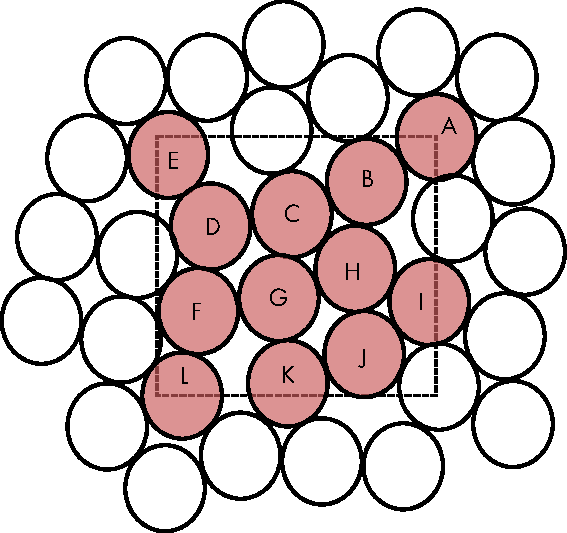
\includegraphics[width=\singleimagewidth]{chapters/figures/void-fraction-cell.pdf}\label{fig:centroid-void-fraction}
\end{figure}
The simplest method for calculating the porosity of a CFD computational cell is to map all the DEM particles into the Eulerian volume via their centroid. We refer to this simple technique as the particle centroid method; in spite of its simplicity it is often used for large cell-to-particle volume ratios.\cite{Xu1997} A two-dimensional demonstration of the centroid technique is given in Fig.~\ref{fig:centroid-void-fraction}. In this figure, we see a computational cell (dashed line) in which many particles exist either partially or fully. The particles shaded in red have their centers located inside the cell and therefore in the simple technique have their entire volume contribute to the calculation of the porosity. The porosity for the centroid method is calculated as,
\begin{equation}
	\epsilon_\text{cell} = 1-\frac{1}{V_\text{cell}}\sum_{i = A}^{i=L}V_{p,i}
\end{equation}
where $V_{p,i}$ is the volume of particle $i$. As the cell size begins to approach the size of the particle, erroneous calculations of porosity arise. This is visible, for instance, when considering particle $A$ in Fig.~\ref{fig:centroid-void-fraction}. This particle has only a quarter of its volume inside the cell but the porosity of the cell is computed as if the entire particle existed inside. Hoomans\etal~recognized this limitation of the centroid method and introduced a fractional volume method.\cite{Hoomans1996} In the fractional volume method, the porosity is found as only partial volumes of the original sphere,
\begin{equation}
	\epsilon_\text{cell} = 1-\frac{1}{V_\text{cell}}\sum_{i = A}^{i=L}f_iV_{p,i}
\end{equation}
where $f_i$ is the fraction of the particle residing in the Eulerian cell. A similar approach taken by Kloss\etal~and Zhao \& Shan is the divided technique.\cite{Kloss2012,Zhao2013a} In this technique, the spherical particle is artificially divided into a number of regions with markers indicating their location. For example, see now how particle $A$ is treated in Fig.~\ref{fig:centroid-void-fraction-divided}. Instead of searching for centroids of particles, each particle has a search through the marker points (the black markers drawn in particle $A$) and the volume of that section of the sphere is assigned to whichever cell it falls inside.
\begin{figure}[t]
	\centering
	\caption{The dashed line represents a computational cell in which exist many particles. The particles with centroids inside the cell are shaded red.}
	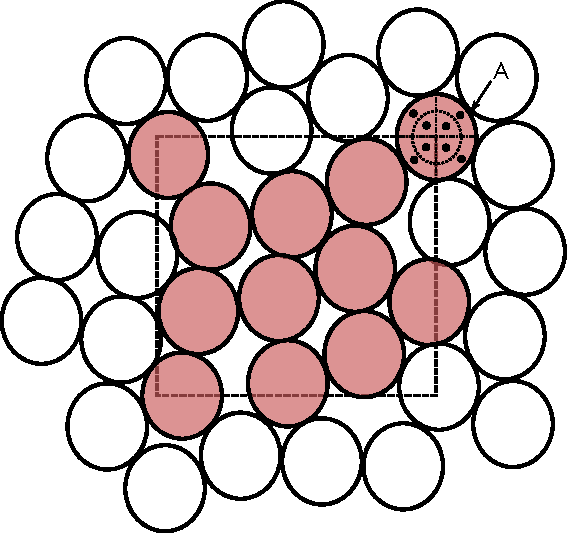
\includegraphics[width=\singleimagewidth]{chapters/figures/void-fraction-divided-cell.pdf}\label{fig:centroid-void-fraction-divided}
\end{figure}

As the computational cell volume approaches the size of a single particle $V_\text{cell}\rightarrow V_p$, the centroid and divided techniques break down. A technique introduced by Link\etal~treats the particle as a porous cube and allows computations when a cell is completely occupied by only a single particle.\cite{Link2005} Peng\etal~offer an an analytic technique as well as guidelines for validity of either analytic or centroid techniques.\cite{Peng2014} However, in this work, I will always apply the divided technique of Kloss\etal~based on the geometry of our packed bed flow and the guidelines established by Peng\etal\cite{Kloss2012,Peng2014}


\subsection{Eulerian-Lagrangian Mapping Calculations of Force and Energy}
Once the fluid momentum and energy fields are calculated in the Eulerian grid, the coupled inter-phase exchange coefficients must map the velocities and temperatures onto the particles in the Lagrangian DEM framework. A particle centroid method is always used in the exchange onto the particles. Referencing Fig.~\ref{fig:centroid-void-fraction}, the velocity and temperature of the dashed cell is mapped only onto the particles highlighted in red. The approach has been used successfully by others.\cite{Xu1997,Link2005,Kloss2012}







\subsection{Discussion on the Applicability of CFD-DEM Governing Equations}
Early work on gas-particle flow models treated the solid and gas phases as two inter-penetrating continuum. The solid and gas were treated with the so-called two fluid model (TFM) by Anderson \& Jackson in 1967.\cite{Anderson1967} The TFM approach is similar to the VAT approach in that the fluid computational cell is sufficiently large to include many individual particles but still smaller than the size of the system.\cite{Enwald1996} The governing equations of TFM are fundamentally similar to Eqs.~\ref{eq:cfd-equations} but required constitutive equations for closure between the fluid and solid phases. Zhou\etal~show the equivalence of the governing equations of TFM and CFD-DEM.\cite{Zhou2010} The essential difference is that the issue of closure is removed with the information from DEM providing direct coupling to the fluid phase.

Since the introduction of the CFD-DEM coupling methodology by Tsuji\etal~in 1993 and then Hoomans\etal~in 1996, many researchers have adopted the approach when particle-scale information of granular and fluidized beds is important.\cite{Tsuji1993,Hoomans1996} Fluidized beds have many industrial applications and are most often studied with coupled CFD-DEM tools. A short example of work can be found in Refs.~\cite{Xu1997,Patankar2001,Swasdisevi2005,Deen2007,Zhang2008,Chu2008,VanBuijtenen2011,Gruber2012,Peng2014}

Noting the growth in application of CFD-DEM, a systematic review of the theoretical developments behind different particular system models was given by Zhu\etal\cite{Zhu2007} They consider the two most common formulations, following the notation of Gidaspow, for the governing equations. The two formulations are commonly referred to simply as Model A and Model B.\cite{gidaspow1994multiphase} Both of these models have been implemented somewhat interchangeably in CFD-DEM simulations. As pointed out by Zhu\etal, the two models differ by their treatment of the pressure drop. In Model A, the pressure drop on the system is jointly shared by the gas and solid phases. In Model B, it is only the gas phase which directly experiences the effects of pressure drop. Therefore, the two models have different forms of coupling source term, $S_k$ (see Eq.~\ref{eq:cfd-mom-source}). The source of Model B is related to that of Model A as $S_k^B = S_k^A/\epsilon - \rho_f\phi g$.

However, as is shown by Zhou\etal, there is a built-in assumption to Model B which is typically overlooked in the implementation of CFD-DEM. For an accelerating fluid, there is an added-mass in the momentum equation. In the derivation of Model B, it is tacitly assumed that the fluid is steady which is not generally valid.\cite{Zhou2010} Nevertheless, the proliferation of Model B is due to the ease in numerical implementation and, except for some situations, Model B is numerically similar to Model A for most cases studied in CFD-DEM simulations.\cite{Zhou2010} In the simulations of packed beds for tritium breeding, we choose to implement Model B as it is valid for any of the flow scenarios ever experienced by the ceramic pebble bed.







% Stability
% viscous momentum does not propagate approximately more than one cell in a single time step. If a characteristic time, $T$, is resolved with $M$ steps, then a fluid packet will travel a distance of $L$ at velocity $U$, $TU = L$. 